\documentclass[a4paper,12pt]{article}

%%% Работа с русским языком
\usepackage{cmap}					% поиск в PDF
\usepackage{mathtext} 				% русские буквы в формулах
\usepackage[T2A]{fontenc}			% кодировка
\usepackage[utf8]{inputenc}			% кодировка исходного текста
\usepackage[english,russian]{babel}	% локализация и переносы
\usepackage{xcolor}
\usepackage{hyperref}
 % Цвета для гиперссылок
\definecolor{linkcolor}{HTML}{799B03} % цвет ссылок
\definecolor{urlcolor}{HTML}{799B03} % цвет гиперссылок

\hypersetup{pdfstartview=FitH,  linkcolor=linkcolor,urlcolor=urlcolor, colorlinks=true}

%%% Дополнительная работа с математикой
\usepackage{amsfonts,amssymb,amsthm,mathtools} % AMS
\usepackage{amsmath}
\usepackage{icomma} % "Умная" запятая: $0,2$ --- число, $0, 2$ --- перечисление

%% Номера формул
%\mathtoolsset{showonlyrefs=true} % Показывать номера только у тех формул, на которые есть \eqref{} в тексте.

%% Шрифты
\usepackage{euscript}	 % Шрифт Евклид
\usepackage{mathrsfs} % Красивый матшрифт

%% Свои команды
\DeclareMathOperator{\sgn}{\mathop{sgn}}

%% Перенос знаков в формулах (по Львовскому)
\newcommand*{\hm}[1]{#1\nobreak\discretionary{}
{\hbox{$\mathsurround=0pt #1$}}{}}
% графика
\usepackage{graphicx}
\graphicspath{{pictures/}}
\DeclareGraphicsExtensions{.pdf,.png,.jpg}
\author{Бурмашев Григорий, БПМИ-208}
\title{Язык SQL, дз -- 7}
\usepackage[left=15mm, top=30mm, right=15mm, bottom=30mm, nohead, nofoot]{geometry}
\date{\today}
\begin{document}
\maketitle
\section*{Номер 1}
\begin{center}

\includegraphics[scale=0.6]{t1.png}
\end{center}
Ориентируясь на следующий отрывок из учебника:
\begin{center}

\includegraphics[scale=0.6]{11.png}
\end{center}
Я полагаю, что операция вставки пройдет успешно, поскольку дело мы имеем с NULL, где по сути NULL != NULL. Т.е два объекта из условия будут сохранять свойство уникальности. Для подтверждения я решил просимулировать условия задачи и посмотреть на результат:
\begin{center}
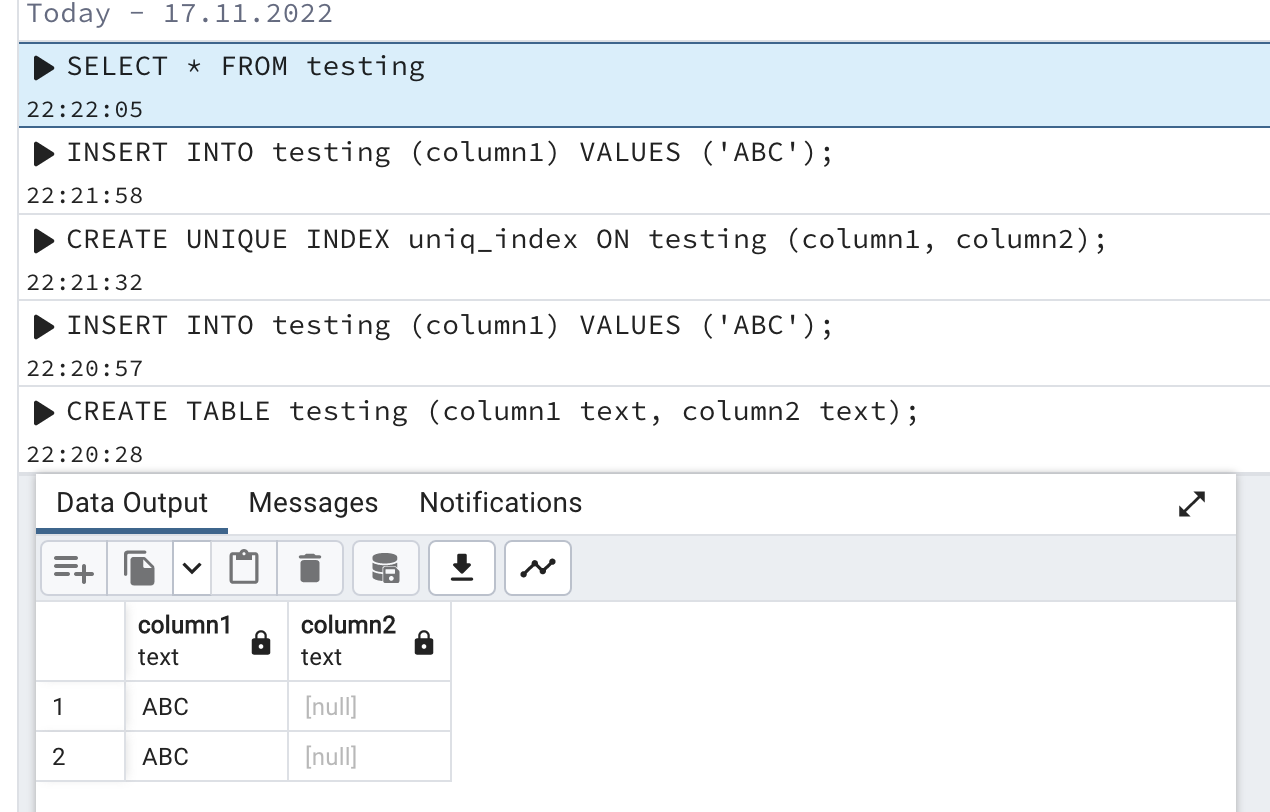
\includegraphics[scale=0.7]{12.png}
\end{center}
Вставка действительно прошла успешно
\clearpage
\section*{Номер 3}
\begin{center}

\includegraphics[scale=0.8]{t2.png}
\end{center}
Для начала я запустил запросы без индекса и посмотрел на их время выполнения, для решения использовал отображение времени в утилите pgAdmin 4.
\begin{itemize}
\item Запрос с типом \textbf{Comfort}:
\begin{center}
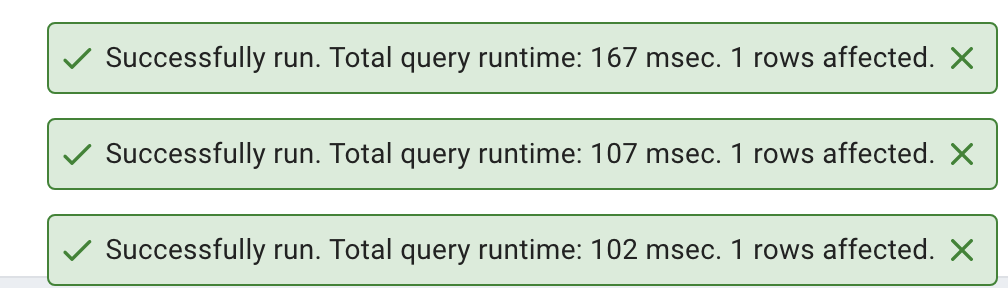
\includegraphics[scale=0.4]{21.png}
\end{center}
\item Запрос с типом \textbf{Business}:
\begin{center}
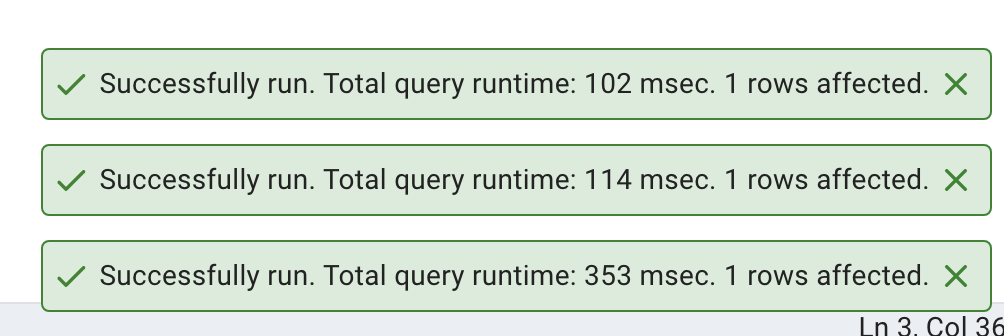
\includegraphics[scale=0.4]{22.png}
\end{center}
\item Запрос с типом \textbf{Economy}:
\begin{center}
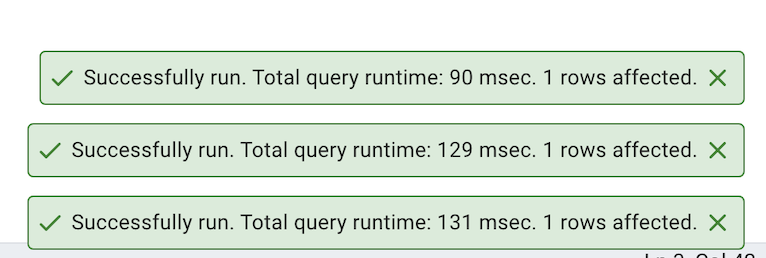
\includegraphics[scale=0.4]{23.png}
\end{center}
\end{itemize}
Различия получились действительно незначительные, только 1 из запусков запроса для типа Business обрабатывался 350 мс, могу посчитать это выбросом. После я создал индекс по fare\_conditions, время получилось:
\begin{itemize}
\item Запрос с типом \textbf{Comfort}:
\begin{center}
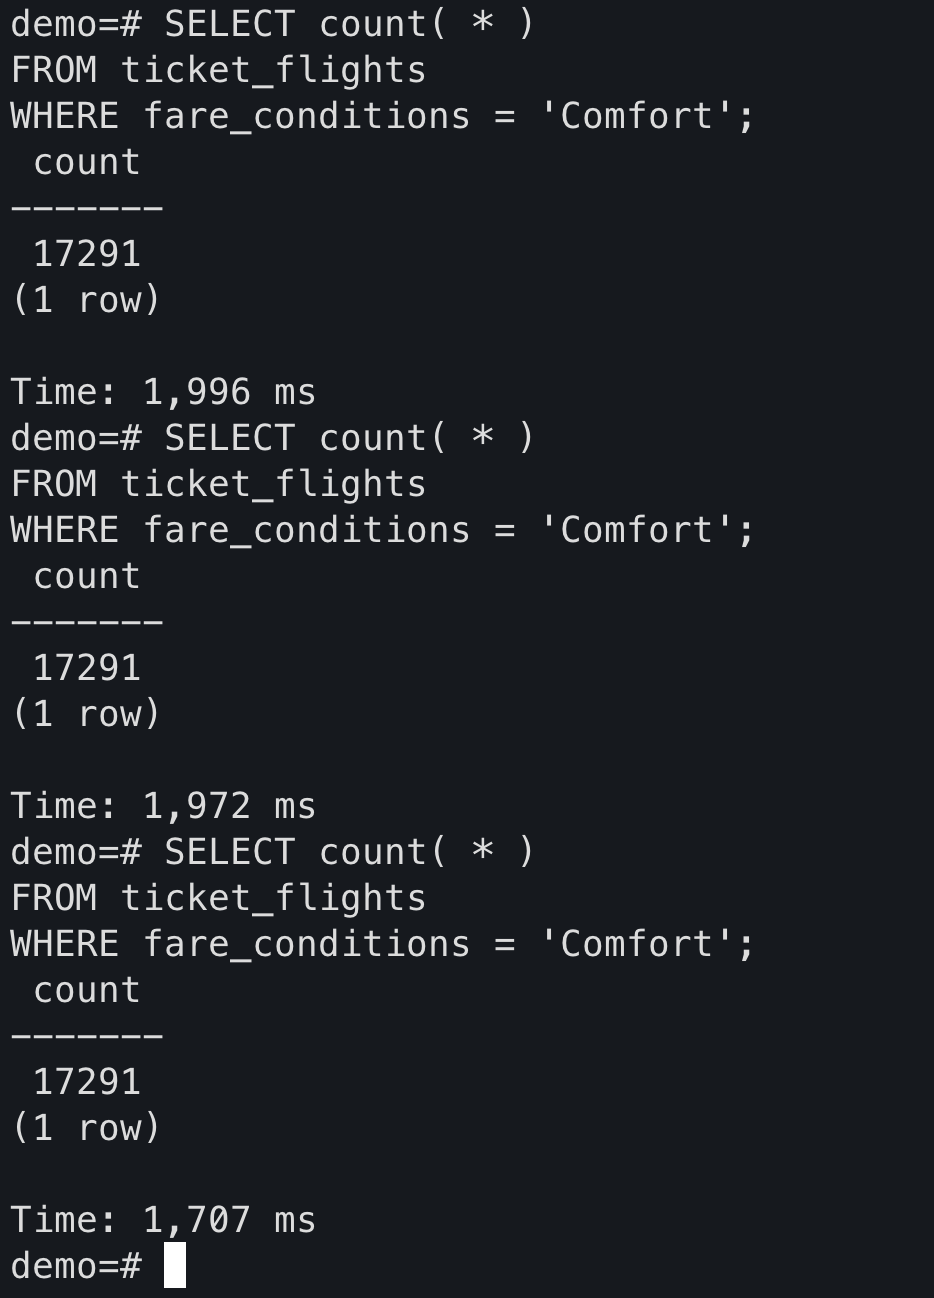
\includegraphics[scale=0.4]{24.png}
\end{center}
\item Запрос с типом \textbf{Business}:
\begin{center}

\includegraphics[scale=0.4]{25.png}
\end{center}
\item Запрос с типом \textbf{Economy}:
\begin{center}
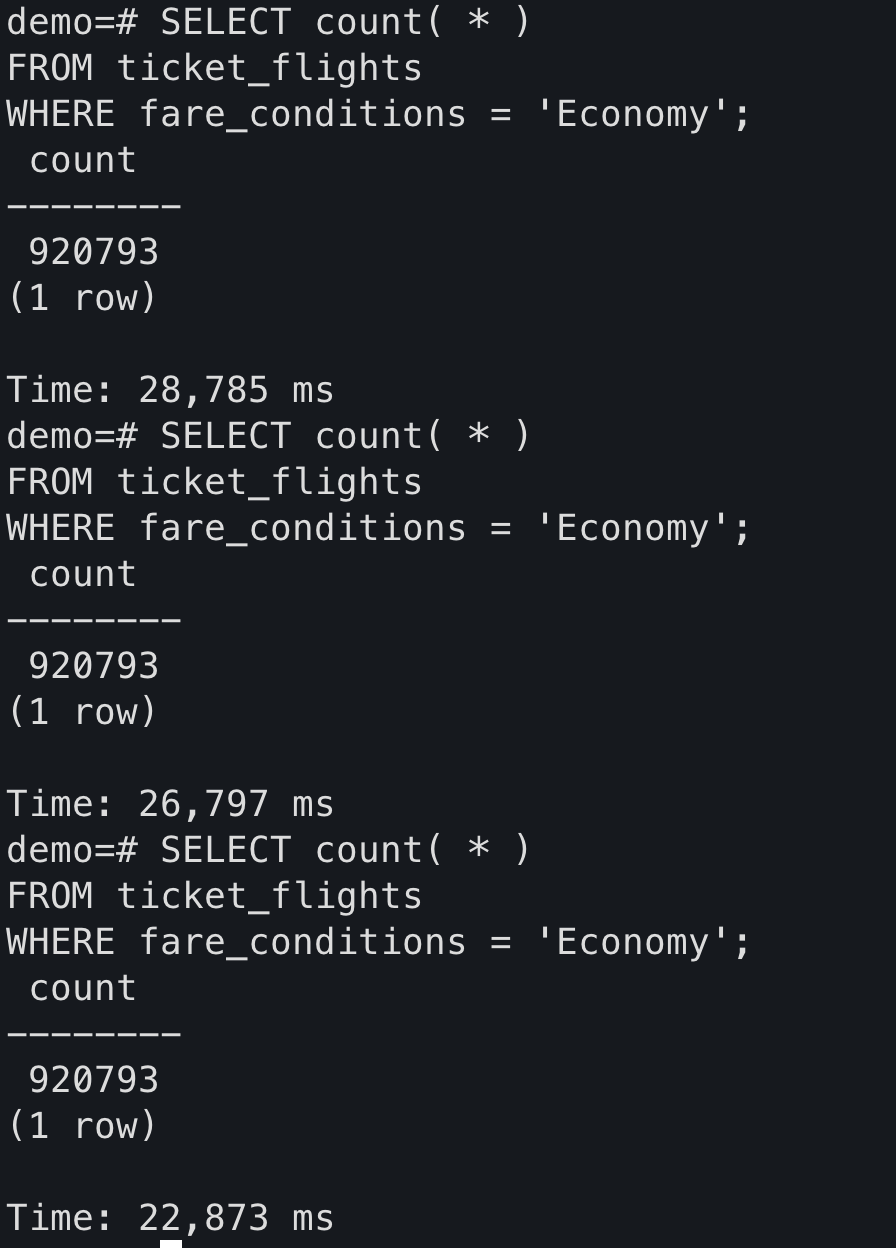
\includegraphics[scale=0.4]{26.png}
\end{center}
\end{itemize}
Очевидный результат, запросы стало выполняться намного быстрее. Для класса \textbf{Economy} время выполнения запросов немного выше, я думаю это связано с бОльшим количеством строк с этим классом, поскольку селективность меньше, а индексы наиболее хорошо работают при высокой селективности.
\end{document}
